\section{Cover decidability}
\label{sec:cover-decidability}

This section is devoted to proving the main result of this paper:

\begin{restatable}{theorem}{decidablecover}
\COVER for \BNRA{}s is decidable. Moreover, the problem is $\Fcomplexity{\omega^\omega}$-complete.
\end{restatable}

Thanks to Proposition~\ref{prop:loc-eq-test-elimination}, we may suppose that our protocols have no $\quotemarks{\eqtestact}$ (the complexity class $\Fomegaomega$ being stable by exponential reduction). 

The intuition of our decidability procedure is as follows. 
Consider a given run and a given agent $a$ that covers some state $q$. We are interested in what the agent needs from other agents to cover $q$. The agent $a$ might need to receive a sequence $w \in \messages^*$ of messages that all have the same value, so that it stores the value of the first such message then tests equality with the stored value upon reception of following messages. 
From the other agents' perspective, this means that someone (or several agents) must broadcast $w$ with the same value in every broadcast. We later call this a \emph{"boss specification"}.  
Moreover, the agent $a$ might first broadcast messages with some value $\aval$ that it had initially and require to receive from other agents messages with this same value $\aval$. 
From the other agent's perspective, this means that someone, after receiving sequence of messages $w$ all with the same value $\aval$, must broadcast a given message $\amessage$ with value $\aval$. We later call this a \emph{"follower specification"}.

The two roles identified previously are the key to the decidability procedure. While, in the original run, it could be that some agent plays several such roles, we will in fact show, thanks to copycat properties, that one might consider that each agent only plays one such role. We will consider a "decomposition trees" where each node provides a witness that a given "role" can be carried out. We will then provide bounds on the size of the "unfolding tree" that we have to consider, and conclude that a decidability procedure can simply guess such a "decomposition tree". 

We will proceed as follows. In \ref{sec:decidability-def}, we introduce several usefuls notions. In \ref{sec:decidability-tree-unfoldings}, we define the notion of "unfolding tree". In \ref{sec:decidability-shortening-branches}, we provide useful arguments towards shortening branches of a tree. In \ref{sec:local-bounds}, we provide useful arguments towards bounding the size of a given node of the tree. In \ref{sec:tree-bounds}, we bound the overall size of the tree. In \ref{sec:decidability-end}, we conclude by proving our decidabily procedure. 

\luin{ajouter ici plan de la section, intuition} %nico: j'en ai mis, à relire et modifier


\subsection{Useful definitions}
\label{sec:decidability-defs}

We first define a notion of "local run", which may be understood as the projection of a "run" onto a given agent. 
	
	A ""local configuration"" is a pair $(q, \localdata) \in Q \times \nats^r$. %Intuitively, it describes the configuration of a single agent. 

	An ""external message"" from $(q,\localdata)$ to $(q',\localdata')$ with transition $\atrans \in \transitions$ and value $\aval \in \nats$, denoted $(q,\localdata) \extbr{\atrans}{\aval} (q',\localdata')$, is defined when $\atrans$ is of the form $(q,\rec{m}{j}{\anact},q')$ with $\localdata(j') = \localdata(j')$ for all $j' \neq j$ and one of the following cases holds:
	
	\begin{minipage}[t]{6cm}
		\begin{itemize}
			\item $\anact = \quotemarks{\dummyact}$ 
			and $\localdata(j) = \localdata'(j)$
			\item $\anact = \quotemarks{\enregact}$ and $\localdata'(j) = v$
		\end{itemize}
	\end{minipage}
	\begin{minipage}[t]{6cm}
		\begin{itemize}
			\item $\anact = \quotemarks{\eqtestact}$ and $\localdata(j) = \localdata'(j)= v$
			\item $\anact = \quotemarks{\diseqtestact}$ and $\localdata(j) = \localdata'(j) \ne v$.
		\end{itemize}
	\end{minipage}
	
	Said otherwise, $(q,\localdata) \extbr{\atrans}{\aval} (q',\localdata')$ when an agent in $(q,\localdata)$ may perform $\atrans$ upon receiving a message of type $\amessage$ and of value $\aval$.

	An ""internal step"" from $(q,\localdata)$ to $(q',\localdata')$ with transition $\atrans \in \transitions$, denoted $(q,\localdata) \intstep{\atrans} (q',\localdata')$, is defined when $\atrans$ is either a "broadcast" or a "local test" and an agent in $(q,\localdata)$ may perform this transition in isolation and get to $(q',\localdata')$. 

	A ""local step"" $(q,\localdata) \step{} (q',\localdata')$ is either an "external message" or an "internal step". 
	A ""local run"" is a sequence $\localrun$ of "local steps" $(q_0, \nu_0) \step{\locallabel_1} (q_1, \nu_1) \step{\locallabel_2} \cdots \step{\locallabel_k} (q_k, \nu_k)$ where, for all $i$, $\locallabel_i \in \set{\extlabel{\atrans}{\aval} \mid \atrans \in \transitions, \aval \in \nats} \cup \set{\intlabel{\atrans} \mid \atrans \in \transitions}$. 
	A ""trace"" is a sequence in $(\set{\extlabel{\atrans}{\aval} \mid \atrans \in \transitions, \aval \in \nats} \cup \set{\intlabel{\atrans} \mid \atrans \in \transitions})^*$. The ""trace"" of a "local run" $\localrun$ is the "trace" $\trace{\localrun}$ containing the message types and values that $\localrun$ receives and broadcasts. Given a "trace" $\atrace$, we write $(q,\localdata) \step{\tau} (q',\localdata')$ to express that there exists a "local run" of "trace" $\atrace$ from $(q,\localdata)$ to $(q',\localdata')$. %peut-être qu'on peut mettre une partie de ça en annexe au niveau de la preuve du lemme tower

	The ""input"" of a "local run" $\localrun$ is the sequence $\Input{\localrun} \in (\messages \times \nats)^*$ containing messages types and values of its "external messages".
	Similarly, its ""output"", which we denote by $\Output{\localrun} \in (\messages \times \nats)^*$, is the sequence of messages of (internal) broadcast steps made in $\localrun$.
	
	Given a value $v \in \nats $, the $v$-input $\vinput{\aval}{\localrun} $(resp. the $v$-output $\voutput{\aval}{\localrun}$) of $\localrun$ is defined as the sequence of messages of $\Input{\localrun}$ (resp. $\Output{\localrun}$) that have value $\aval$. Formally, $\vinput{\aval}{\localrun}$ is the word $m_0 \cdots m_{\ell} \in \messages^*$ such that $(m_0, \aval) \cdots (m_{\ell}, \aval)$ is the projection of $\Input{\localrun}$ on $\messages \times \set{\aval}$. 


\subsection{Unfolding trees}
\label{sec:decidability-tree-unfoldings}

Consider an agent $a$ that initially has value $\aval$ in one of its registers. After broadcasting some word $w$ with value $\aval$, $a$ may need some other agent to broadcast $\amessage_1$ with value $\aval$. An agent doing so did not have $\aval$ initially, hence it may be cloned at will: we are able to send $\amessage_1$ with value $\aval$ as many times as we want. Then, if $a$, after broadcasting $w_2$ with value $\aval$, must receive a message $\amessage_2$ with value $\aval$, then the agent broadcasting $\amessage_2$ may receive with value $\aval$ a word of the form $w_1 \cdot w_2'$ where $w_2'$ is $w_2$ where some $\amessage_1$ were inserted. Similarly, if $a$ then needs $\amessage_3$ with value $\aval$ after broadcasting $w_3$, then an agent playing that role may beforehand receive with value $\aval$ a word of the form $w_1 \cdot w_2'' \cdot w_3''$ where $w_2''$ is $w_2$ where some $\amessage_1$ were inserted, and $w_3''$ is $w_3$ where some $\amessage_2$ and $\amessage_3$ were inserted. We formalize this observation using "decompositions":

A ""decomposition"" is a tuple $\decsymb = (w_0, m_1, \ldots, m_\ell, w_\ell)$ with $w_0, \ldots, w_\ell \in \messages^*$, and $m_1, \cdots, m_\ell \in \messages$, with $m_i \neq m_j$ for all $i\neq j$. In particular we have $\ell \leq \size{\messages}$. 

We say that $w \in \messages^*$ ""admits decomposition"" $\decsymb = (w_0, m_1, \ldots, m_\ell, w_\ell)$ if $w \subword w'_0 w'_1 \cdots w'_\ell$ where for all $j$, $w'_j$ can be obtained from $w_j$ by adding letters from $\set{m_1, \ldots, m_{j-1}}$.
We denote by $\langdec{\decsymb}$ the language of words that admit decomposition $\decsymb$. 

We may now formally define our "unfolding trees" which abstractly represent executions. 
An ""unfolding tree"" $\tree$ over $\prot$ is
a finite tree where each node $\node$ has three labels:
\begin{itemize}
	\item The first one is a local run of $\prot$, written $\localrunlabel{\node}$. 
	
	\item The second one is a value, written $\valuelabel{\node}$.
	
	\item The third one is a ""specification"" $\speclabel{\node}$, which is either a word $\bosslabel{\node} \in \messages^*$ (""boss specification"") or a pair $(\followlabelword{\node}, \followlabelmessage{\node}) \in \messages^* \times \messages$ (""follower specification""). In the first case we say that the node is a ""boss node"", otherwise it is a ""follower node"".
\end{itemize} 

Before stating the conditions that the tree must satisfy, we provide a bit of intuition. Let $\node$ a node of $\tree$; let $\aval := \valuelabel{\node}$ and $\localrun := \localrunlabel{\node}$. In this tree, the children of a local run are the witnesses that this local run may be turned into a real run, as they provide the messages received in the local run. To satisfy a boss specification $\bossspec$, one must certify that $\bossspec$ may be sent with value $\aval$; to do so, \nicoin{todo}


\begin{itemize}
	\item[C1\namedlabel{unfoldingC1}{C1}] If it is a "boss node" then:
	\begin{itemize} 
		\item $\aval$ is an initial value of $\localrun$, 
		\item there exists a "decomposition" $\decsymb = (w_0, m_1, w_1, \ldots, m_{\ell}, w_{\ell})$ such that $\bosslabel{\node} \in \langdec{\decsymb}$, 
		\item $\localrun$ may be split into successive "local runs" $\localrun_0, \dots, \localrun_{\ell}$ where, for all $i \in \nset{1}{\ell}$, $w_i \subword \voutput{\aval}{\localrun_i}$ and $\vinput{\aval}{\localrun_i} \in \set{m_1, \dots, m_{i-1}}^*$, and
		\item  for all $i \in [1,\ell]$, $\node$ has a child $\node_i$ which is a "follower node" such that $\followlabelmessage{\node_i} = m_i$ and $\followlabelword{\node_i} \in\langdec{\decsymb_i}$ where $\decsymb_i = (w_0, m_1, w_1, \ldots, m_{i-1}, w_{i-1})$.
	\end{itemize}
	\item[C2\namedlabel{unfoldingC2}{C2}] If $\node$ is a "follower node" then $\aval$ is not an initial value of $\localrun$, $\vinput{\aval}{\localrun} = \followlabelword{\node}$ and 
	$\voutput{\aval}{\localrun}$ contains $\followlabelmessage{\node}$.
	
	\item[C3\namedlabel{unfoldingC3}{C3}] In both cases, for all value $\aval' \neq \aval$ broadcast or received at some point in $\localrunlabel{\node}$, one of the two following conditions is satisfied:
	\begin{itemize}
		\item[C3.1\namedlabel{unfoldingC3.1}{C3.1}]
			$\aval$ is an initial value of $\localrun$, 
		there exists $\decsymb' = (w'_0, m'_1, w'_1, \ldots, m'_{\ell'}, w'_{\ell'})$, s.t. $\localrun$ may be split into sucessive "local runs" $\localrun'_0, \dots, \localrun'_{\ell}$ where, for all $i \in \nset{1}{\ell'}$, $\voutput{\aval'}{\localrun'_i} \subword w'_i$ and $\vinput{\aval'}{\localrun'_i} \in \set{m'_0, \dots, m'_{i-1}}^*$, and
		for all $i \in\nset{1}{\ell'}$, $\node$ has a child $\node'_i$ which is a "follower node" such that $\followlabelmessage{\node'_i} = m'_i$ and $\followlabelword{\node'_i} \in\langdec{\decsymb'_i}$ where $\decsymb'_i = (w'_0, m'_1, w'_1, \ldots, m'_{i-1}, w'_{i-1})$.
		%  If $\aval'$ is an initial value of $\localrun$ then there exists a "decomposition" $\decsymb' = (w'_0, m'_1, w'_1, \ldots, m'_k, w'_k)$ 
		% where $w'_0 w'_1 \ldots w'_k = \voutput{\aval'}{\localrunlabel{\node}}$, for all $j \in \nset{1}{k}$ all receptions of $m'_j$ with value $\val'$ in $u$ happen after the broadcasts of $w'_0\cdots w'_{j-1}$ with value $\val'$, and for all $j \in [1,k]$ $\node$ has a child $\node'$ which is a "follower node" such that $\followlabelmessage{\node'} = m'_j$ and $\followlabelword{\node'} \in\langdec{\decsymb'_j}$ where $\decsymb'_j = (w_0, m_1, w_1, \ldots, m_{j-1}, w_{j-1})$.  
		
		\item[C3.2\namedlabel{unfoldingC3.2}{C3.2}] If $\aval'$ is not an initial value of $\localrun$ then $\node$ has a child $\node'$ which is a "boss node" such that $\vinput{\aval'}{\localrun}$ is a subword of $\bosslabel{\node'}$.
	\end{itemize}
\end{itemize}


%Old def

%\begin{definition}
%	\label{def:tree-unfolding}
%	A ""unfolding tree"" is
%	a finite tree where each node has three labels:
%	\begin{itemize}
%		\item The first one is a local run of $\prot$. 
%		
%		\item The second one is a value $v \in \nats$.
%		
%		\item The third one is a ""specification"", which is either a word $bw \in \messages^*$ or a pair $(fw, fm)$ with $fm \in \messages$ and $fw \in \messages^*$ a "decomposition". In the first case we say that the node is a ""boss node"", otherwise it is a ""follower node"". 
%	\end{itemize} 
%	
%	It must satisfy the following conditions:
%	Let $\node$ be a node of that tree, and $u$ and $v$ the local run and value labelling it. The following conditions must hold:
%	
%	\begin{itemize}
%		\item[C1\namedlabel{unfoldingC1}{C1}] If it is a "boss node" labelled by $w \in \messages^*$ then $v$ is an initial value of $u$ and there exists a decomposition $\decsymb = (w_0, m_1, w_1, \ldots, m_{\ell}, w_{\ell})$ such that
%		$w_0 \cdots w_\ell$ is the $v$-output of $u$, $w \in \langdec{\decsymb}$, and for all $j \in \nset{1}{\ell}$, $\node$ has a child which is a "follower node" with a label $\decsymb \subword ((w_0, m_1, w_1, \ldots, m_{j-1}, w_{j-1}), m_j)$.
%		
%		\item[C2\namedlabel{unfoldingC2}{C2}] If it is a "follower node" labelled $(\decsymb, m)$ then $v$ is not an initial value of $u$, the $v$-input of $u$ is in $\langdec{\decsymb}$, and $m$ is broadcast at some point in $u$ with value $v$.
%		
%		\item[C3\namedlabel{unfoldingC3}{C3}] In both cases, for all $v' \neq v$ broadcast or received at some point in $u$,
%		\begin{itemize}
%			\item[C3.1\namedlabel{unfoldingC3.1}{C3.1}] If $v'$ is an initial value of $u$ then there exists a "decomposition" $\decsymb' = (w'_0, m'_1, w'_1, \ldots, m'_k, w'_k)$ where $w'_0 w'_1 \ldots w'_k$ is the $v'$-output of $u$, for all $j \in \nset{1}{k}$ all receptions of $m_j$ with value $v'$ in $u$ happen after the broadcasts of $w'_0\cdots w'_{j-1}$ with value $v'$, and for all $j \in \nset{1}{k}$ $\node$ has a child which is a "follower node" with a label $\decsymb \subword ((w_0, m_1, w_1, \ldots, m_{j-1}, w_{j-1}), m_j)$.  
%			
%			\item[C3.2\namedlabel{unfoldingC3.2}{C3.2}] If $v'$ is not an initial value of $u$ then $\node$ has a child which is a "boss node" labelled by $w'$ such that $\vinput{v}{u}$ is a subword of $w'$.
%		\end{itemize}
%	\end{itemize}
%	
%	
%\end{definition}


%\begin{remark}
% The conditions \ref{unfoldingC1}, \ref{unfoldingC2} and \ref{unfoldingC3} defined in Definition~\ref{def:tree-unfolding} only depend on the
%\end{remark}


\begin{definition}
	A "run" $\run$ satisfies a boss specification $\bossspec$ if there exists $\aval \in \nats$ such that $\bossspec$ is a subword of the sequence of messages sent with value $\aval$ through $\run$.
	
	A "run" $\run$ satisfies a follower specification $(\followwordspec, \followmessagespec)$ if there exists a value $\aval$ and an agent $a$ such that $\aval$ is not an initial value of $a$, the $\aval$-input of $a$ in $\run$ is a subword of $\followwordspec$ and agent $a$ broadcasts $\followmessagespec$ with value $\aval$ at some point.
	
	An "unfolding tree" satisfies a boss specification $\bossspec$ if its root $\node$ is a "boss node" and $\bossspec$ is a subword of its specification label $\bosslabel{\node}$.
	An "unfolding tree" satisfies a follower specification $(\followwordspec, \followmessagespec)$ if its root $\node$ is a "follower node" such that $\followmessagespec=\followlabelmessage{\node}$ and  $\followlabelword{\node}$ is a subword of $\followwordspec$.
\end{definition}

We will now prove that there exists a run satisfying a specification if and only if there exists a finite tree satisfying that same specification. To do so, we will build a tree from a run and conversely.


Also note that the interpretation of the "follower nodes" changes between the two directions: when building the tree a follower node labelled $(\followwordspec, \followmessagespec)$ means that there exists a global run in which some agent receives the sequence of messages $\followwordspec$ and broadcasts $\followmessagespec$, all with a value $\aval$ that is not one of its initial ones.
\nico{pas clair}

When building the run a follower node means that there exists a "partial run" which receives a sequence of external messages which forms the word $fw$, with a value $v$ that it initially does not contain, and eventually broadcasts $m$ with that same value.

\begin{restatable}{lemma}{LemRunToTree}
	\label{lem:run-to-tree}
	Let $\prot$ be a protocol.
	If there exists a finite run $\run$ of $\prot$ satisfying some "specification" $\spec$ then there exists a finite "unfolding tree" $\tree$ labelled with local runs of $\prot$ satisfying $\spec$. \nico{pourquoi label par $\prot$?}
\end{restatable}

\begin{restatable}{lemma}{LemTreeToRun}
	\label{lem:tree-to-run}
	Let $\prot$ be a "protocol".
	If there exists a finite "unfolding tree" labelled by local runs of $\prot$ satisfying a "boss specification" $bw \in \messages^*$ then there exists  a finite "run" $\run$ of $\prot$ satisfying $bw$.
\end{restatable}

The proof can be found in Appendix~\ref{app:tree-to-run}.



\subsection{Shortening branches}
\label{sec:decidability-shortening-branches}

\begin{restatable}{lemma}{lemIncreasingBosses}
	\label{lem:increasing-bosses}
	Let $\tree$ be a "unfolding tree" satisfying a specification $\spec$.
	Let $\node, \node'$ be two "boss nodes" of $\tree$.
	If $\node$ is an ancestor of $\node'$ and $\bosslabel{\node}$ is a subword of $\bosslabel{\node'}$ then there exists a smaller "unfolding tree" satisfying $\spec$.  
\end{restatable}

\begin{restatable}{lemma}{lemIncreasingFollowers}
	\label{lem:increasing-followers}
	Let $\tree$ be a "unfolding tree" satisfying a specification $\spec$.
	Let $\node, \node'$ be two "follower nodes" of $\tree$.
	If $\node$ is an ancestor of $\node'$, $\followlabelword{\node'} \subword \followlabelword{\node}$ and $\followlabelmessage{\node'}=\followlabelmessage{\node}$ then there exists a smaller "unfolding tree" satisfying $\spec$. 
\end{restatable}


\subsection{Local bounds}
\label{sec:local-bounds}


\begin{figure}
	

	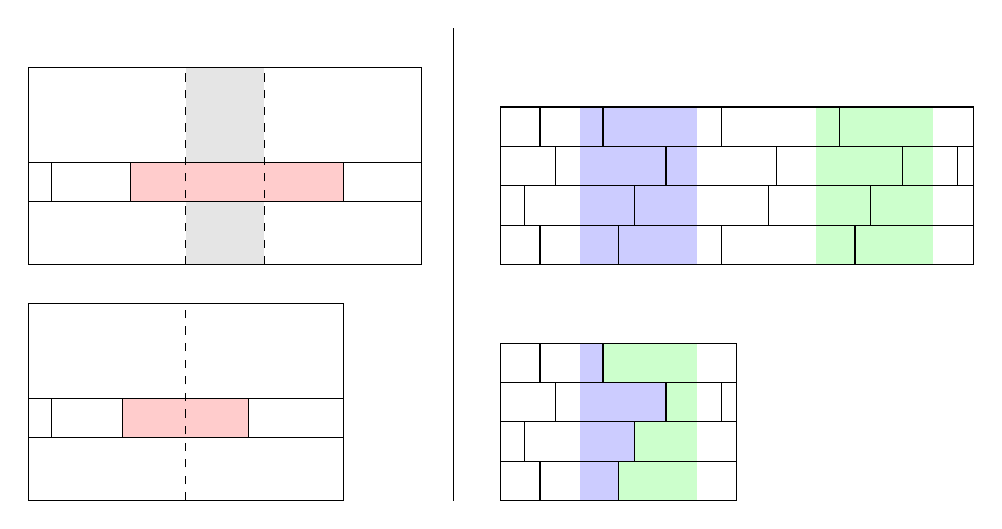
\begin{tikzpicture}
		\draw[white,fill=gray!20] (2,0) rectangle (3,0.8);
		\draw[white,fill=gray!20] (2,1.3) rectangle (3,2.5);
		
		\draw (0,0) rectangle (5,2.5);
		
		\draw (0,0.8) rectangle (5,1.3);
		
		\draw (0,0.8) rectangle (0.3,1.3);
		\draw (0,0.8) rectangle (1.3,1.3);
		\draw[fill=red!20] (1.3,0.8) rectangle (4,1.3);
		
		\draw[dashed] (2,0) -- (2,2.5);
		\draw[dashed] (3,0) -- (3,2.5);
		
		
		
		\draw (0,-3) rectangle (4,-0.5);
		
		\draw (0,-2.2) rectangle (4,-1.7);
		
		\draw (0,-2.2) rectangle (0.3,-1.7);
		\draw (0.3,-2.2) rectangle (1.3,-1.7);
		\draw[fill=red!20] (1.2,-2.2) rectangle (2.8,-1.7);
		
		\draw[dashed] (2,-3) -- (2,-0.5);
		
		\draw (5.4,-3) -- (5.4,3);
		
		
		\draw[white,fill=blue!20] (7,0) rectangle (8.5,2);
		\draw[white,fill=green!20] (10,0) rectangle (11.5,2);
		
		\draw (6,0) rectangle (12,2);
		
		\draw (6,0) rectangle (12,0.5);
		\draw (6,0) rectangle (12,1);
		\draw (6,0) rectangle (12,1.5);
		
		\draw (6,0) rectangle (6.5,0.5);
		\draw (6,0) rectangle (7.5,0.5);
		\draw (6,0) rectangle (8.8,0.5);
		\draw (6,0) rectangle (10.5,0.5);
		
		\draw (6,0.5) rectangle (6.3,1);
		\draw (6,0.5) rectangle (7.7,1);
		\draw (6,0.5) rectangle (9.4,1);
		\draw (6,0.5) rectangle (10.7,1);
		
		\draw (6,1) rectangle (6.7,1.5);
		\draw (6,1) rectangle (8.1,1.5);
		\draw (6,1) rectangle (9.5,1.5);
		\draw (6,1) rectangle (11.1,1.5);
		\draw (6,1) rectangle (11.8,1.5);
		
		\draw (6,1.5) rectangle (6.5,2);
		\draw (6,1.5) rectangle (7.3,2);
		\draw (6,1.5) rectangle (8.8,2);
		\draw (6,1.5) rectangle (10.3,2);
		
		
		\draw[white, fill=blue!20] (7,-3) rectangle (7.5,-2.5);
		\draw[white,fill=blue!20] (7,-2.5) rectangle (7.7,-2);
		\draw[white,fill=blue!20] (7,-2) rectangle (8.1,-1.5);
		\draw[white,fill=blue!20] (7,-1.5) rectangle (7.3,-1);
		
		\draw[white,fill=green!20] (7.5,-3) rectangle (8.5,-2.5);
		\draw[white,fill=green!20] (7.7,-2.5) rectangle (8.5,-2);
		\draw[white,fill=green!20] (8.1,-2) rectangle (8.5,-1.5);
		\draw[white,fill=green!20] (7.3,-1.5) rectangle (8.5,-1);
		
		
		
		\draw (6,-3) rectangle (9,-2.5);
		\draw (6,-3) rectangle (9,-2);
		\draw (6,-3) rectangle (9,-1.5);
		\draw (6,-3) rectangle (9,-1);
		
		\draw (6,-3) rectangle (6.5,-2.5);
		\draw (6,-3) rectangle (7.5,-2.5);
		
		\draw (6,-2.5) rectangle (6.3,-2);
		\draw (6,-2.5) rectangle (7.7,-2);
		
		\draw (6,-2) rectangle (6.7,-1.5);
		\draw (6,-2) rectangle (8.1,-1.5);
		\draw (6,-2) rectangle (8.8,-1.5);
		
		\draw (6,-1.5) rectangle (6.5,-1);
		\draw (6,-1.5) rectangle (7.3,-1);
		
	\end{tikzpicture}


	\caption{Illustration of the proof of Lemma~\ref{lem:short-local-runs}. We represent local runs as above, where Lines correspond to registers, and vertical separations are times at which a $\enregact$ operation is performed on that register. If one register $i$ keeps the same value for a long enough time (on the left), we apply the induction hypothesis to shorten the projection of the run on the other registers. As the value of $i$ does not change, the resulting run is still valid. If all registers change values often, say every $M$ steps (on the right), then if the run is long enough we can find two identical sequences of transitions during which all values are renewed twice. We can then obtain a shorter run by glueing them together as in the picture. The colored rectangles in the shortened runs correspond to fresh values that we introduce to make sure that all local disequality tests succeed.}
\end{figure}
\begin{restatable}{lemma}{lemShortLocalRuns}
	\label{lem:short-local-runs}
	There exists a function $\towerfun(n) (\regnum)$ in $O(\intro*\repexp{n}{\regnum})$ such that, for every protocol $\prot$ with $r$ registers per process, for every "local run" $\localrun: (q, \localdata) \step{*} (q', \localdata')$ in $\prot$, for every $V \subseteq \nats$ finite that contains every message value appearing in $\localrun$, there exists $\localrun': (q, \localdata) \step{*} (q', \localdata')$\corto{uniformiser la notation} such that $\length{\localrun'} \leq \towerfun(\size{\prot})(r)$ and:
	\begin{enumerate}
		\item \label{item:shorterrun_anyvalue} for all $\aval' \in \nats$, there exists $\aval \in \nats$ such that $\vinput{\aval'}{\localrun'}$ is a subword of $\vinput{\aval}{\localrun}$,
		\item \label{item:shorterrun_oldvalues} for all $\aval \in V$, $\vinput{\aval}{\localrun'}$ is a subword of $\vinput{\aval}{\localrun}$. 
		% \item by writing $V := \nats \setminus \set{\localdata_i(k) \mid k \in \nset{1}{\regnum}}$, for every $\aval' \in V$, there exists $\aval \in V$ such that $\vinput{\aval'}{\localrun'}$ is a subword of $\vinput{\aval}{\localrun}$.
	\end{enumerate}
		%  with an "input" $I$.
% 	Let $u_1, u_2, u_3$ be such that $u=u_1u_2u_3$.
% 	If $\size{u_2} > TOWER$, then there exists $u'_2$ with $|u_2'| \leq \towerfun(\prot)$ such that $u_1u'_2u_3$ is a local run of $\prot$ with smaller "input" than $u$. 
\end{restatable}

\begin{remark}
	The tower bound of Lemma~\ref{lem:short-local-runs} is tight, in the sense that some local runs may need to have length a tower of exponentials of linear height in the number of registers.
	It also holds for pushdown automata, and for all transition systems which have some kind of pumping lemma.
	\cortoin{To formalize}
\end{remark}


\begin{restatable}{lemma}{lemShortRunOutput}
	\label{lem:short-run-for-output}
	For every protocol $\prot$ with $r$ registers per process, for every $w_{in} \in (\messages\times \nats)^*$, if there exists a "local run" $\localrun: (q, \localdata) \step{*} (q', \localdata')$ in $\prot$ such that $w_{in} \subword \Output{\localrun}$, then for every $V \subseteq \nats$ finite that contains every message value appearing in $\localrun$, there exists $\localrun': (q, \localdata) \step{*} (q', \localdata')$ such that $\length{\localrun'} \leq (\towerfun(\size{\prot})(r)+1)\size{w_{in}}$, $w_{in} \subword \Output{\localrun'}$ and:
	
	\begin{enumerate}
		\item for all $\aval' \in \nats$, there exists $\aval \in \nats$ such that $\vinput{\aval'}{\localrun'}$ is a subword of $\vinput{\aval}{\localrun}$,
		\item for all $\aval \in V$, $\vinput{\aval}{\localrun'}$ is a subword of $\vinput{\aval}{\localrun}$. 
	\end{enumerate}
\end{restatable}


\begin{restatable}{lemma}{lemBoundSuccessorHeight}
	\label{lem:bound-successor-height}
	Let $\prot$ be a "protocol", let $\node$ be a node of a "unfolding tree" $\tree$ of minimal size labelled by $\prot$ satisfying a "boss specification" $w$.
	Let $\node_1, \ldots, \node_k$ be its "follower" children. If $\node$ is not the root of $\tree$ then let $\mu'$ be its father.
	We have the following properties:
	
	\begin{enumerate}
		\item $k \leq \size{\messages}r$ 
		
		\item The root of $\tree$ is a "boss node".
				
		\item  If $\node$ is a "boss node" then 
		\begin{itemize}
			\item If $\node$ is the root of $\tree$ then $\bosslabel{\node} = w$
			
			\item If $\node$ is not the root then $\size{\bosslabel{\node}} \leq \size{\localrunlabel{\node'}}$
			
			\item In both cases $\size{\localrunlabel{\node}} \leq (\towerfun(\size{\prot})(r) + 1)\Big[ \size{\bosslabel{\node}} + \sum_{i=1}^k \size{\followlabelword{\node_i}} \Big]$
		\end{itemize}
	
		\item If $\node$ is a "follower node" then 
		\begin{itemize}			
			\item $\size{\followlabelword{\node}} \leq \size{\localrunlabel{\node}}$
			
			\item $\size{\localrunlabel{\node}} \leq (\towerfun(\size{\prot})(r) +1)\Big[ 1 + \sum_{i=1}^k \size{\followlabelword{\node_i}} \Big]$
			
		\end{itemize}
	\end{enumerate}
\end{restatable}


\subsection{Tree bounds}
\label{sec:tree-bounds}

\begin{definition}
	We define the ""altitude"" of a node $\node$, written $\altitude{\node}$, in a "unfolding tree" recursively as follows:
	\begin{itemize}
		\item The altitude of the root is $0$
		
		\item The altitude of a "boss node" is the altitude of its father minus one
		
		\item The altitude of a "follower node" is the altitude of its father plus one.
	\end{itemize}
\end{definition}

\begin{restatable}{lemma}{lemBoundLengthHeightH}
	\label{lem:bound-length-at-height-h}
	Let $\prot$ be a protocol, let $\node$ be a node of a "unfolding tree" of minimal size labelled by $\prot$ satisfying a "boss specification" $w$.
	Let $\altmax$ be the maximal "altitude" in $\tau$, let $N = \size{w} + \size{\prot} +1$ and let $f_0 : \nats \to \nats$ be the function mapping each $n \in \nats$ to $f_0(n)=(N^2 (\towerfun(N)(N) + 1))^{n+1}$ 
	
	\begin{itemize}
		\item If $\node$ is a "boss node" then $\size{\bosslabel{\node}} \leq f_0(\altmax - \altitude{\node}-1)$ and $\size{\localrunlabel{\node}} \leq f_0(\altmax - \altitude{\node})$.
		
		\item If $\node$ is a "follower node" then $\size{\localrunlabel{\node}} \leq \size{\followlabelword{\node}} \leq  f_0(\altmax - \altitude{\node})$.
	\end{itemize} 
\end{restatable}

\begin{restatable}{lemma}{lemBoundMaxHeight}
	\label{lem:bound-max-height}
	There exists a function $f_1$ of the class $\Ffunction{\omega^{\size{\messages}}}$ such that for all "protocol" $\prot$, for all "unfolding tree" $\tree$ of minimal size labelled by $\prot$ satisfying a "boss specification" $w$, the maximal altitude of a node of $\tree$ is bounded by $f_1(\size{\prot} + \size{w}+1)$.
\end{restatable}


\begin{restatable}{lemma}{lemBoundMinHeight}
	\label{lem:bound-min-height}
	There exists a function $f_2$ of the class $\Ffunction{\omega^{\size{\messages}+1}}$ such that for all "protocol" $\prot$, for all "unfolding tree" $\tree$ of minimal size labelled by $\prot$ satisfying a "boss specification" $w$, the absolute value of the minimal "altitude" of a node of $\tree$ is bounded by $f_2(\size{\prot} + \size{w}+1)$.
\end{restatable}



\begin{corollary}
	\label{cor:bound-node-size}
	There exists a function $f_3$ of the class $\Ffunction{\omega^{\size{\messages}+1}}$\corto{corriger les M en M+1} such that for all "protocol" $\prot$, for all "unfolding tree" $\tree$ of minimal size labelled by $\prot$ satisfying a "boss specification" $w$, for all node $\node$ of $\tree$,
	
		\begin{itemize}
		\item $\size{\localrunlabel{\node}} \leq f_3(\size{\prot}+ \size{w})$
			
		\item If $\node$ is a "boss node" then $\size{\bosslabel{\node}} \leq f_3(\size{\prot}+ \size{w})$.
		
		\item If $\node$ is a "follower node" then $\size{\followlabelword{\node}} \leq f_3(\size{\prot}+ \size{w})$.
	\end{itemize} 
\end{corollary}

\ifproofs
\begin{proof}
	Consequence of Lemmas~\ref{lem:bound-length-at-height-h}, \ref{lem:bound-max-height} and \ref{lem:bound-min-height} as $\Ffunction{\omega^{\size{\messages}+1}}$ is closed by composition with elementary functions.
\end{proof}
\fi
\begin{restatable}{proposition}{PropBoundTreeSize}
	\label{prop:bound-tree-size}
	There exists a function $f_4$ of the class $\Ffunction{\omega^{\size{\messages}+1}}$ such that for all "protocol" $\prot$, for all "unfolding tree" $\tree$ of minimal size labelled by $\prot$ satisfying a "boss specification" $w$, the size of $\tree$ is bounded by $f_4(\size{\prot} + \size{w}+1)$.
\end{restatable}




\subsection{Decidability}
\label{sec:decidability-end}


\ifproofs
\begin{proof}
	The lower bound is given by the reduction from "lossy channel systems" reachability in Proposition~\ref{prop:reduction-LCS}.
	
	For the upper bound, let $\prot$ be a "protocol" with $\regnum \geq 1$ registers over messages $\messages$ and $q$ one of its states. We add a new message $m$ to $\messages$ and a new transition $\br{m}{1}$ from $q$ to itself broadcasting $m$. 
	Clearly the new "protocol" $\prot'$ satisfies the "boss specification" $m$ if and only if $q$ is coverable in $\prot$.
	
	By Lemmas~\ref{lem:run-to-tree} and \ref{lem:tree-to-run}, there is a run of $\prot'$ satisfying $m$ if and only if there is a "unfolding tree" satisfying $m$.
	By Lemma~\ref{prop:bound-tree-size}, there is such a "unfolding tree" if and only if there is one of size at most $f_4(\size{\prot}+2)$, where $f_4$ is a function of the class $\Ffunction{\omega^{\size{\messages}}}$.
	
	The last problem we have is that the size of a "unfolding tree" does not take into account the values used in it. This can be solved by noticing that the conditions in the definition of a "unfolding tree" and the condition to satisfy a "specification" still hold after applying an injective renaming to the values. 
	
	Suppose there exists $\tree$ a "unfolding tree" satisfying $m$, let $V$ be the set of values appearing in that tree. In a node $\node$ the values appearing are $\valuelabel{\node}$, the initial values of $\localrunlabel{\node}$ (there are $r$ such values), the non-initial values (at most $\size{\localrunlabel{\node}}$ as they all need to be received).
	Hence there are at most $\size{\localrunlabel{\node}} + r +1$ different values appearing in each node.
	In total there are thus at most $\sum_{\node \in \tree} \size{\localrunlabel{\node}} + r +1$ different values in $\tree$, which is less than $(r+2)\size{\tree}$.
	
	We can apply an injective renaming $V \to \nset{1}{(r+2)\size{\tree}}$ to the values to obtain another "unfolding tree" satisfying $m$ and whose values do not exceed $(r+2)\size{\tree}$.
	As a result, there exists a "unfolding tree" satisfying $m$ if and only if there is one of size at most $f_4(\size{\prot}+2)$ in which values do not exceed $f_4(\size{\prot}+2)$. A description of such a tree requires a space that is polynomial in its size.
	
	We can therefore bound the size of the description of such a "unfolding tree" by a function of $\Ffunction{\omega^{\size{\messages}}}$.
	An algorithm for the coverability problem thus consists in enumerating all trees labelled by local runs of $\prot$ of size at most $f_4(\size{\prot}+2)$ with values not exceeding $f_4(\size{\prot}+2)$, and accepting if and only if one of them satisfies the conditions to be a "unfolding tree" satisfying $m$.
	This can all be done in exponential time in $f_4(\size{\prot}+2)$, thus this algorithm terminates in time $f_5(\size{\prot})$ where $f_5$ is a function of $\Ffunction{\omega^{\size{\messages}}}$.
	
	The BNRA coverability problem is thus decidable in time $\Ffunction{\omega^\omega}$.
\end{proof}
\fi
